\documentclass[tikz,convert={density=150,size=600,outext=.png}]{standalone}
\usetikzlibrary{shapes, calc, arrows, fit, positioning, decorations, patterns, decorations.pathreplacing, chains, snakes}

\begin{document}
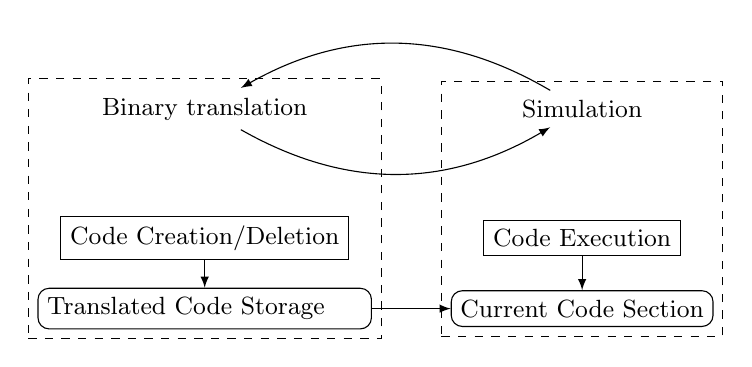
\begin{tikzpicture}[>=latex, font=\small]
\matrix[column sep=1cm, row sep=0.1cm]{
    \node (bt) {Binary translation}; & \node (sim) {Simulation}; \\[1.cm]
    \node[draw] (translation) {Code Creation/Deletion}; & \node[draw] (execution) {Code Execution}; \\[0.25cm]
    \node[draw, rounded corners,text width=4cm, align=left] (storage) {Translated Code Storage}; & \node[draw, rounded corners] (current-page) {Current Code Section}; \\
};
\draw[->] (bt) to [bend right] (sim);
\draw[->] (sim) to [bend right] (bt);
\draw[->] (storage) to (current-page);
\draw[->] (translation) -- (storage);
\draw[->] (execution) -- (current-page);

\node[draw, dashed, fit = (bt) (translation) (storage)] {};
\node[draw, dashed, fit = (sim) (execution) (current-page)] {};

\end{tikzpicture}
\end{document}
